\documentclass[]{tufte-handout}

% ams
\usepackage{amssymb,amsmath}

\usepackage{ifxetex,ifluatex}
\usepackage{fixltx2e} % provides \textsubscript
\ifnum 0\ifxetex 1\fi\ifluatex 1\fi=0 % if pdftex
  \usepackage[T1]{fontenc}
  \usepackage[utf8]{inputenc}
\else % if luatex or xelatex
  \makeatletter
  \@ifpackageloaded{fontspec}{}{\usepackage{fontspec}}
  \makeatother
  \defaultfontfeatures{Ligatures=TeX,Scale=MatchLowercase}
  \makeatletter
  \@ifpackageloaded{soul}{
     \renewcommand\allcapsspacing[1]{{\addfontfeature{LetterSpace=15}#1}}
     \renewcommand\smallcapsspacing[1]{{\addfontfeature{LetterSpace=10}#1}}
   }{}
  \makeatother

\fi

% graphix
\usepackage{graphicx}
\setkeys{Gin}{width=\linewidth,totalheight=\textheight,keepaspectratio}

% booktabs
\usepackage{booktabs}

% url
\usepackage{url}

% hyperref
\usepackage{hyperref}

% units.
\usepackage{units}


\setcounter{secnumdepth}{2}

% citations

% pandoc syntax highlighting
\usepackage{color}
\usepackage{fancyvrb}
\newcommand{\VerbBar}{|}
\newcommand{\VERB}{\Verb[commandchars=\\\{\}]}
\DefineVerbatimEnvironment{Highlighting}{Verbatim}{commandchars=\\\{\}}
% Add ',fontsize=\small' for more characters per line
\newenvironment{Shaded}{}{}
\newcommand{\AlertTok}[1]{\textcolor[rgb]{1.00,0.00,0.00}{\textbf{#1}}}
\newcommand{\AnnotationTok}[1]{\textcolor[rgb]{0.38,0.63,0.69}{\textbf{\textit{#1}}}}
\newcommand{\AttributeTok}[1]{\textcolor[rgb]{0.49,0.56,0.16}{#1}}
\newcommand{\BaseNTok}[1]{\textcolor[rgb]{0.25,0.63,0.44}{#1}}
\newcommand{\BuiltInTok}[1]{#1}
\newcommand{\CharTok}[1]{\textcolor[rgb]{0.25,0.44,0.63}{#1}}
\newcommand{\CommentTok}[1]{\textcolor[rgb]{0.38,0.63,0.69}{\textit{#1}}}
\newcommand{\CommentVarTok}[1]{\textcolor[rgb]{0.38,0.63,0.69}{\textbf{\textit{#1}}}}
\newcommand{\ConstantTok}[1]{\textcolor[rgb]{0.53,0.00,0.00}{#1}}
\newcommand{\ControlFlowTok}[1]{\textcolor[rgb]{0.00,0.44,0.13}{\textbf{#1}}}
\newcommand{\DataTypeTok}[1]{\textcolor[rgb]{0.56,0.13,0.00}{#1}}
\newcommand{\DecValTok}[1]{\textcolor[rgb]{0.25,0.63,0.44}{#1}}
\newcommand{\DocumentationTok}[1]{\textcolor[rgb]{0.73,0.13,0.13}{\textit{#1}}}
\newcommand{\ErrorTok}[1]{\textcolor[rgb]{1.00,0.00,0.00}{\textbf{#1}}}
\newcommand{\ExtensionTok}[1]{#1}
\newcommand{\FloatTok}[1]{\textcolor[rgb]{0.25,0.63,0.44}{#1}}
\newcommand{\FunctionTok}[1]{\textcolor[rgb]{0.02,0.16,0.49}{#1}}
\newcommand{\ImportTok}[1]{#1}
\newcommand{\InformationTok}[1]{\textcolor[rgb]{0.38,0.63,0.69}{\textbf{\textit{#1}}}}
\newcommand{\KeywordTok}[1]{\textcolor[rgb]{0.00,0.44,0.13}{\textbf{#1}}}
\newcommand{\NormalTok}[1]{#1}
\newcommand{\OperatorTok}[1]{\textcolor[rgb]{0.40,0.40,0.40}{#1}}
\newcommand{\OtherTok}[1]{\textcolor[rgb]{0.00,0.44,0.13}{#1}}
\newcommand{\PreprocessorTok}[1]{\textcolor[rgb]{0.74,0.48,0.00}{#1}}
\newcommand{\RegionMarkerTok}[1]{#1}
\newcommand{\SpecialCharTok}[1]{\textcolor[rgb]{0.25,0.44,0.63}{#1}}
\newcommand{\SpecialStringTok}[1]{\textcolor[rgb]{0.73,0.40,0.53}{#1}}
\newcommand{\StringTok}[1]{\textcolor[rgb]{0.25,0.44,0.63}{#1}}
\newcommand{\VariableTok}[1]{\textcolor[rgb]{0.10,0.09,0.49}{#1}}
\newcommand{\VerbatimStringTok}[1]{\textcolor[rgb]{0.25,0.44,0.63}{#1}}
\newcommand{\WarningTok}[1]{\textcolor[rgb]{0.38,0.63,0.69}{\textbf{\textit{#1}}}}

% longtable
\usepackage{longtable,booktabs}

% multiplecol
\usepackage{multicol}

% strikeout
\usepackage[normalem]{ulem}

% morefloats
\usepackage{morefloats}


% tightlist macro required by pandoc >= 1.14
\providecommand{\tightlist}{%
  \setlength{\itemsep}{0pt}\setlength{\parskip}{0pt}}

% title / author / date
\title{TP1 - Reconocimiento de Patrones}
\author{Elio Campitelli}
\date{4/17/2020}


\begin{document}

\maketitle




\hypertarget{generar-set-de-datos}{%
\section{Generar set de datos}\label{generar-set-de-datos}}

Para cada x, los datos a generear siguen una distribución \(p(x, y) = \mathcal{N}(\mu = \sin(2\pi x), \sigma = 0.3)\). Esta función de densidad de probabilidad conjunta se muestra en la Figura \ref{fig:densidad}. El mejor ajuste en el sentido de cuadrados mínimos está dado por \(\mathrm{h}(x) = \mathbb{E}(y|x) =\sin(2\pi x)\). Ambas funciones (\(p(x, y)\) y \(\mathbb{E}(y|x)\)) se grafican en la Figura \ref{fig:densidad}.

\begin{figure}
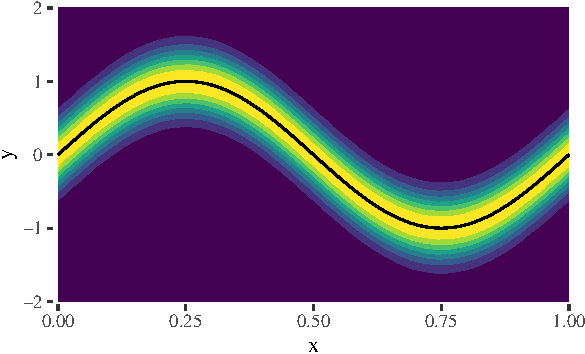
\includegraphics{README_files/figure-latex/densidad-1} \caption{Densidad de probabilidad conjunta $p(x, y) = \mathcal{N}(\sin(2\pi x), 0.3)$. En negro, la línea $\mathbb{E}(y|x)$.}\label{fig:densidad}
\end{figure}

La función \texttt{D}\footnote{Definida en el \protect\hyperlink{def-d}{Apéndice}.} devuelve \texttt{L} sets de \texttt{n} datos. Éstos corresponden a la función \texttt{FUN} (default: \(\sin(2\pi x)\))) evaluada en \texttt{n} puntos elegidos a partir de una distribución uniforme en el intervalo \texttt{intervalo} (default: \((0, 1)\)) a la que se le suma un ruido gausiano con media 0 y desvío \texttt{sigma} (default: \(0.3\)).

\begin{figure}
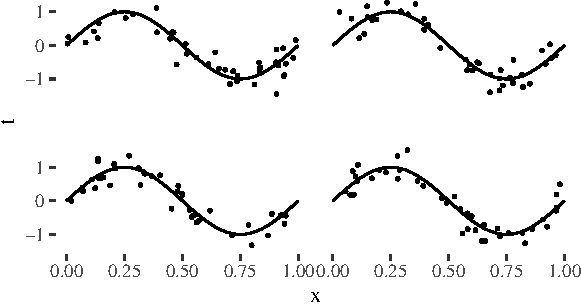
\includegraphics{README_files/figure-latex/unnamed-chunk-2-1} \caption[Cuatro ejemplos de conjuntos de datos generados por la función `D` con `n = 40`]{Cuatro ejemplos de conjuntos de datos generados por la función `D` con `n = 40`. En línea negra, la función $t = \sin(2\pi x)$}\label{fig:unnamed-chunk-2}
\end{figure}

\hypertarget{funciuxf3n-para-calcular-la-regresiuxf3n}{%
\subsection{Función para calcular la regresión}\label{funciuxf3n-para-calcular-la-regresiuxf3n}}

\texttt{regresion\_poly}\footnote{Definida en el \protect\hyperlink{def-regr}{Apéndice}.} tiene argumentos \texttt{orden} y \texttt{lambda} y devuelve una función que realiza el ajuste polinomial correspondiente\footnote{Esto es una complicación extra pero vale la pena para poder usar la función como argumento de \texttt{method} en \texttt{geom\_smooth()} como se ve en la figura siguiente.}. Los métodos \texttt{predictdf} y \texttt{predict}\footnote{Definidos en el \protect\hyperlink{def-regr}{Apéndice}.} aplican el ajuste a nuevos datos.

La Figura \ref{fig:ajustes-orden} muestra el efecto de cambiar el orden del polinomio para un set de datos de \texttt{n\ =\ 10}. Un polinomio de orden cero es una constante, por lo que el valor predicho por ese ajuste coincide con el promedio muestral. Polinomio de orden 1 agrega una tendencia, y órdenes mayores van aumentando los grados de libertad del modelo. Para órdenes altos (cercanos a la cantidad de datos usados para realizar el ajuste), el modelo es lo suficientemente complejo para predecir los datos observados con gran exactitud, pero pierde poder de generalización para datos no observados.

\begin{figure}
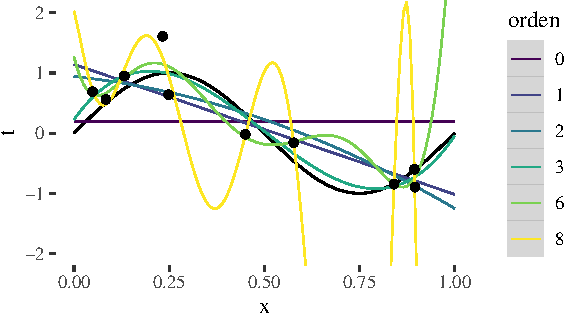
\includegraphics{README_files/figure-latex/ajustes-orden-1} \caption[Ajustes polinomiales con distintos órdenes y lambda = 0 para 1 ejemplo]{Ajustes polinomiales con distintos órdenes y lambda = 0 para 1 ejemplo. La línea negra representa la función real. Al aumentar el grado del polinomio, el ajuste se acerca más a los puntos observados pero oscila alocadamente lejos de ellos.}\label{fig:ajustes-orden}
\end{figure}

En cambio, la Figura \ref{fig:ajustes-lambda} muestra el efecto de aumentar el factor de regularización lambda. Al aumentar, aumenta la penalización de coeficientes altos y el modelo deja de ajustar tan bien a los datos observados pero mejora la generalización.

\begin{figure}
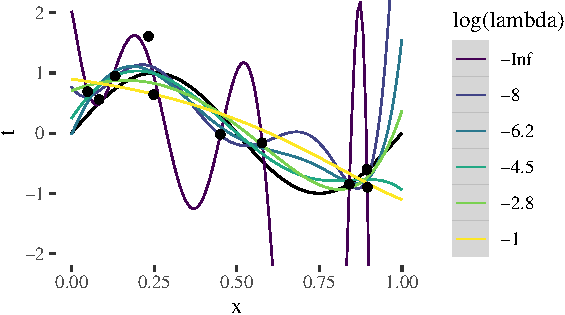
\includegraphics{README_files/figure-latex/ajustes-lambda-1} \caption[Igual que la figura anterior, pero con orden fijo = 8 y lambda variable]{Igual que la figura anterior, pero con orden fijo = 8 y lambda variable. Al aumentar el factor de regularización, el modelo se simplifica. Aumenta la diferencia con los datos usados para el ajuste, pero mejora la generalización.}\label{fig:ajustes-lambda}
\end{figure}

El error cuadrático medio de entrenamiento se calcula como la diferencia cuadrática media entre los valores observados y los predichos por el modelo. En la Figura \ref{fig:rmse-sd} se muestra un histograma de la raiz cuadrada del error cuadrático medio\footnote{RMSE: Root Mean Square Error} para 200 muestras de \texttt{n\ =\ 10} haciendo un ajuste con \texttt{orden\ =\ 3} y \texttt{lambda\ =\ 1e-3}. En el recuadro, el valor medio del RMSE y su desvío estándar.

\begin{figure}
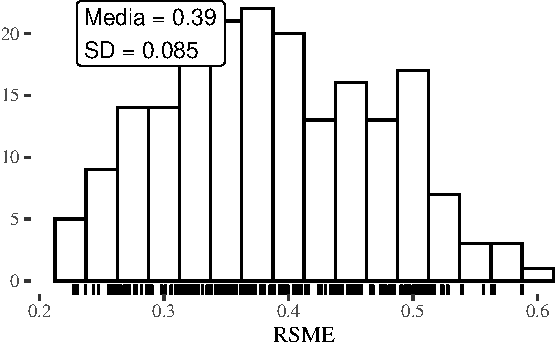
\includegraphics{README_files/figure-latex/rmse-sd-1} \caption[Histograma de la raiz del error cuadrático medio computado para 200 muestras de `n = 10`]{Histograma de la raiz del error cuadrático medio computado para 200 muestras de `n = 10`.}\label{fig:rmse-sd}
\end{figure}

\hypertarget{determinando-m-y-lambda}{%
\subsection{Determinando M y lambda}\label{determinando-m-y-lambda}}

Para elegir el orden y el lambda se puede usar validación cruzada. Para cada combinación de los hiperpaŕametros se separa los datos en un conjunto de \emph{entrenamiento} que se usa para ajustar un modelo y uno de \emph{validación}, que se usa para evaluar el error del modelo a datos nuevos. Se busca la combinación que minimice el error de validación y finalmente se estima el error esperado con el conjunto de \emph{test}.

Esta es la matriz de parámetros donde voy a buscar. Lambda entre 10\^{}-10 y 1, y el orden del polinomio entre 0 y 11

Defino una función para calcular el RSME de validación cruzada\footnote{Definida en el \protect\hyperlink{def-cv}{Apéndice}.}. Ésta toma un set de datos, una formula que determina el modelo y una función de regresión (lo que devuelve \texttt{regresion\_poly()}). Tiene un argumento \texttt{k\_fold} (default: 5) que controla la cantidad de cachos. Si \texttt{k\_fold\ =\ n}, el algoritmo se reduce a LOOCV\footnote{Leave One Out Cross-Validation. Es decir, que se ajusta el modelo usando todos los datos menos uno.}

De los 200 sets de 10 datos voy a usar 150 para la validación cruzada. Luego, para cda uno de ellos voy a hacer validación cruzada con \texttt{k\_fold\ =\ 5}, lo que implica usar 8 datos para el ajuste y 2 para la validación. Este proceso devuelve 150 valores de RMSE de validación cruzada para cada combinación de lambda y orden del polinomio.

La Figura \ref{fig:rmse-campo} muestra la mediana del RMSE de validación cruzada\footnote{La distribución del RMSE es asimétrica, por lo que el promedio no es una medida de distribución central particularmente buena.} para los valores de lambda y orden. La variación del error refleja lo visto en las figuras \ref{fig:ajustes-orden} y \ref{fig:ajustes-lambda}, alcanzando el máximo cuando el orden el polinomio es muy grande y el factor de regularización es muy pequeño (overfitting).

\begin{figure}
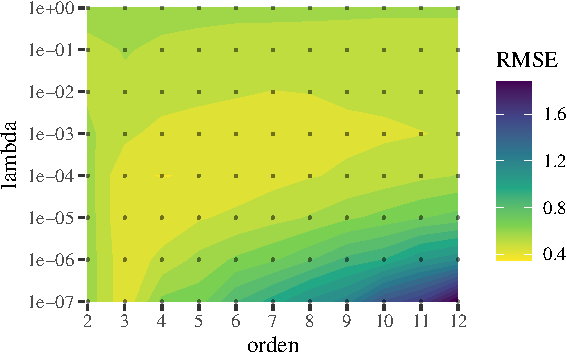
\includegraphics{README_files/figure-latex/rmse-campo-1} \caption[Mediana del RMSE para cada lambda y orden]{Mediana del RMSE para cada lambda y orden.}\label{fig:rmse-campo}
\end{figure}

\begin{table}

\caption{\label{tab:rmse-mejores}Combinación de valores de lambda y orden que minimizan la mediana del RMSE de validación cruzada}
\centering
\begin{tabular}[t]{rrr}
\toprule
lambda & orden & mediana\\
\midrule
1e-04 & 4 & 0.384\\
1e-05 & 3 & 0.385\\
1e-04 & 5 & 0.387\\
1e-04 & 3 & 0.389\\
1e-07 & 3 & 0.407\\
\bottomrule
\end{tabular}
\end{table}

A partir de estos datos se puede elegir la mejor combinación de lambda y orden. La Tabla \ref{tab:rmse-mejores} lista las 5 combinaciones con menor RMSE de validación cruzada medido por la mediana. Según esta medida, la mejor combinación de hiperparámetros es lambda = \ensuremath{10^{-4}}, orden = 4. Para tener una idea de la robustez de esta determinación, en la Figura \ref{fig:rmse-orden} se ordenan las combinaciones de hiperparámetros de menor a mayor de acuerdo a la mediana del RMSE pero también se muestra el intervalo de 95\% en sombreado. Se observa que la variabilidad del RMSE dentro de cada combinación de hiperparámetros es considerablemente mayor que la variabilidad de la mediana del RMSE entre distintas combinaciones de hiperparámetros.

\begin{figure}
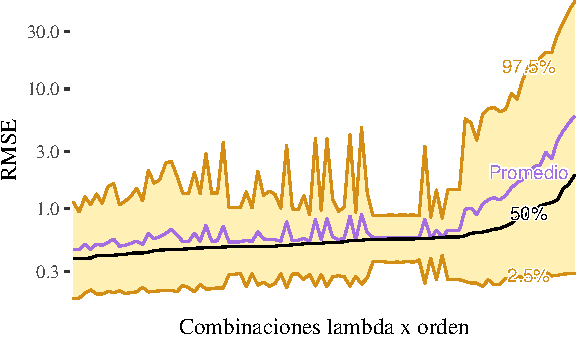
\includegraphics{README_files/figure-latex/rmse-orden-1} \caption[Mediana (en negro) y promedio (en violeta) del RMSE de validación cruzada e intervalo de confianza de 95\%]{Mediana (en negro) y promedio (en violeta) del RMSE de validación cruzada e intervalo de confianza de 95\%. Datos ordenados de menor a mayor a partir de la mediana del RMSE.}\label{fig:rmse-orden}
\end{figure}

Una vez elegida la combinación óptima de hiperparámetros (Tabla \ref{tab:rmse-mejores}) lo que sigue es usarlos para ajustar el modelo con todos los 150 sets de datos usados para validación cruzada y luego testear el RMSE de test usando los 50 sets de datos que habían quedado separados para test. La distribución de RSME obtenida se ve en la Figura \ref{fig:rmse-test}.

\begin{figure}
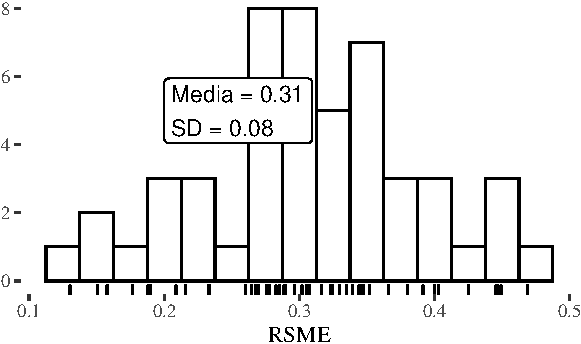
\includegraphics{README_files/figure-latex/rmse-test-1} \caption[Histograma del RSME de test de los 50 sets de datos no utilizados para validación cruzada]{Histograma del RSME de test de los 50 sets de datos no utilizados para validación cruzada.}\label{fig:rmse-test}
\end{figure}

\newpage

\hypertarget{apuxe9ndice}{%
\section{Apéndice}\label{apuxe9ndice}}

\hypertarget{def-d}{%
\subsection{Definición de D}\label{def-d}}

\begin{Shaded}
\begin{Highlighting}[]
\NormalTok{D <-}\StringTok{ }\ControlFlowTok{function}\NormalTok{(}\DataTypeTok{n =} \DecValTok{10}\NormalTok{, }\DataTypeTok{L =} \DecValTok{1}\NormalTok{, }\DataTypeTok{intervalo =} \KeywordTok{c}\NormalTok{(}\DecValTok{0}\NormalTok{, }\DecValTok{1}\NormalTok{), }\DataTypeTok{FUN =} \OperatorTok{~}\KeywordTok{sin}\NormalTok{(}\DecValTok{2}\OperatorTok{*}\NormalTok{pi}\OperatorTok{*}\NormalTok{.x), }\DataTypeTok{sigma =} \FloatTok{0.3}\NormalTok{) \{}
\NormalTok{  datos <-}\StringTok{ }\KeywordTok{lapply}\NormalTok{(}\KeywordTok{seq_len}\NormalTok{(L), }\ControlFlowTok{function}\NormalTok{(l) \{}
\NormalTok{    x <-}\StringTok{ }\KeywordTok{runif}\NormalTok{(n, intervalo[}\DecValTok{1}\NormalTok{], intervalo[}\DecValTok{2}\NormalTok{])}
\NormalTok{    FUN <-}\StringTok{ }\NormalTok{purrr}\OperatorTok{::}\KeywordTok{as_mapper}\NormalTok{(FUN)}
\NormalTok{    real <-}\StringTok{ }\KeywordTok{FUN}\NormalTok{(x)}
\NormalTok{    t <-}\StringTok{ }\NormalTok{real }\OperatorTok{+}\StringTok{ }\KeywordTok{rnorm}\NormalTok{(n, }\DataTypeTok{sd =}\NormalTok{ sigma)}
    \KeywordTok{return}\NormalTok{(data.table}\OperatorTok{::}\KeywordTok{data.table}\NormalTok{(x, t))}
\NormalTok{  \})}
  
  \KeywordTok{return}\NormalTok{(data.table}\OperatorTok{::}\KeywordTok{rbindlist}\NormalTok{(datos, }\DataTypeTok{idcol =} \StringTok{"l"}\NormalTok{))}
\NormalTok{\}}
\end{Highlighting}
\end{Shaded}

\hypertarget{def-regr}{%
\subsection{Definición de regresion\_poly y métodos}\label{def-regr}}

\begin{Shaded}
\begin{Highlighting}[]
\NormalTok{regresion_poly <-}\StringTok{ }\ControlFlowTok{function}\NormalTok{(}\DataTypeTok{orden =} \DecValTok{1}\NormalTok{, }\DataTypeTok{lambda =} \DecValTok{0}\NormalTok{) \{}
  \KeywordTok{force}\NormalTok{(orden)}
  \KeywordTok{force}\NormalTok{(lambda)}
  
\NormalTok{  modelos <-}\StringTok{ }\NormalTok{data.table}\OperatorTok{::}\KeywordTok{CJ}\NormalTok{(orden, lambda)}
  
  \ControlFlowTok{function}\NormalTok{(formula, }\DataTypeTok{data =} \OtherTok{NULL}\NormalTok{, weights) \{}
\NormalTok{    datos <-}\StringTok{ }\KeywordTok{model.frame}\NormalTok{(formula, }\DataTypeTok{data =}\NormalTok{ data)}
\NormalTok{    y <-}\StringTok{ }\NormalTok{datos[, }\DecValTok{1}\NormalTok{]}
\NormalTok{    x <-}\StringTok{ }\NormalTok{datos[, }\DecValTok{2}\NormalTok{]}
\NormalTok{    Ws <-}\StringTok{ }\KeywordTok{lapply}\NormalTok{(}\KeywordTok{seq_len}\NormalTok{(}\KeywordTok{nrow}\NormalTok{(modelos)), }\ControlFlowTok{function}\NormalTok{(i) \{}
\NormalTok{      orden <-}\StringTok{ }\NormalTok{modelos}\OperatorTok{$}\NormalTok{orden[i]}
\NormalTok{      lambda <-}\StringTok{ }\NormalTok{modelos}\OperatorTok{$}\NormalTok{lambda[i]}
      \CommentTok{# Matriz de diseño}
      
      \ControlFlowTok{if}\NormalTok{ (orden }\OperatorTok{==}\StringTok{ }\DecValTok{0}\NormalTok{) \{}
\NormalTok{        A <-}\StringTok{ }\KeywordTok{cbind}\NormalTok{(}\KeywordTok{rep}\NormalTok{(}\DecValTok{1}\NormalTok{, }\KeywordTok{length}\NormalTok{(x)))}
\NormalTok{      \} }\ControlFlowTok{else}\NormalTok{ \{}
\NormalTok{        A <-}\StringTok{ }\KeywordTok{cbind}\NormalTok{(}\DecValTok{1}\NormalTok{, }\KeywordTok{poly}\NormalTok{(x, }\DataTypeTok{degree =}\NormalTok{ orden, }\DataTypeTok{raw =} \OtherTok{TRUE}\NormalTok{))  }
\NormalTok{      \}}
      
      \ControlFlowTok{if}\NormalTok{ (lambda }\OperatorTok{!=}\StringTok{ }\DecValTok{0}\NormalTok{) \{}
\NormalTok{        L <-}\StringTok{ }\KeywordTok{diag}\NormalTok{(}\DecValTok{1}\NormalTok{, }\DataTypeTok{nrow =} \KeywordTok{ncol}\NormalTok{(A)) }\OperatorTok{*}\StringTok{ }\NormalTok{lambda}
\NormalTok{        w <-}\StringTok{ }\KeywordTok{solve}\NormalTok{(}\KeywordTok{t}\NormalTok{(A) }\OperatorTok\StringTok{ }\NormalTok{A }\OperatorTok{+}\StringTok{ }\NormalTok{L) }\OperatorTok\StringTok{ }\KeywordTok{t}\NormalTok{(A) }\OperatorTok\StringTok{ }\NormalTok{y   }\CommentTok{# Forma a lo bruto.}
\NormalTok{      \} }\ControlFlowTok{else}\NormalTok{ \{}
\NormalTok{        w <-}\StringTok{ }\KeywordTok{qr.coef}\NormalTok{(}\KeywordTok{qr}\NormalTok{(A), y)   }\CommentTok{# Forma eficiente de invertir la matriz}
\NormalTok{      \}}
      
\NormalTok{      modelo <-}\StringTok{ }\KeywordTok{list}\NormalTok{(}\DataTypeTok{orden =}\NormalTok{ orden,}
                     \DataTypeTok{lambda =}\NormalTok{ lambda,}
                     \DataTypeTok{w =}\NormalTok{ w)}
      \KeywordTok{return}\NormalTok{(modelo)}
\NormalTok{    \})}
    
    \KeywordTok{attr}\NormalTok{(Ws, }\StringTok{"x"}\NormalTok{) <-}\StringTok{ }\NormalTok{x}
    \KeywordTok{class}\NormalTok{(Ws) <-}\StringTok{ }\KeywordTok{c}\NormalTok{(}\StringTok{"regression_models"}\NormalTok{, }\KeywordTok{class}\NormalTok{(Ws))}
    \KeywordTok{return}\NormalTok{(Ws)}
\NormalTok{  \}}
\NormalTok{\}}
\end{Highlighting}
\end{Shaded}

\begin{Shaded}
\begin{Highlighting}[]
\CommentTok{# Métodos para predecir nuevos valores usando la regresion.}
\NormalTok{predict.regression_models <-}\StringTok{ }\ControlFlowTok{function}\NormalTok{(object, }\DataTypeTok{newdata =} \OtherTok{NULL}\NormalTok{, }\DataTypeTok{which =} \DecValTok{1}\NormalTok{) \{}
  \CommentTok{# browser()}
  \ControlFlowTok{if}\NormalTok{ (}\KeywordTok{is.null}\NormalTok{(newdata)) \{}
\NormalTok{    newdata <-}\StringTok{ }\KeywordTok{attr}\NormalTok{(object, }\StringTok{"x"}\NormalTok{, }\DataTypeTok{exact =} \OtherTok{TRUE}\NormalTok{)}
\NormalTok{  \}}
  
\NormalTok{  model <-}\StringTok{ }\NormalTok{object[[which]]}
  
  \ControlFlowTok{if}\NormalTok{ (model}\OperatorTok{$}\NormalTok{orden }\OperatorTok{==}\StringTok{ }\DecValTok{0}\NormalTok{) \{}
\NormalTok{    A <-}\StringTok{ }\KeywordTok{cbind}\NormalTok{(}\KeywordTok{rep}\NormalTok{(}\DecValTok{1}\NormalTok{, }\KeywordTok{length}\NormalTok{(newdata))) }
\NormalTok{  \} }\ControlFlowTok{else}\NormalTok{ \{}
\NormalTok{    A <-}\StringTok{ }\KeywordTok{cbind}\NormalTok{(}\DecValTok{1}\NormalTok{, }\KeywordTok{poly}\NormalTok{(newdata, }\DataTypeTok{degree =}\NormalTok{ model}\OperatorTok{$}\NormalTok{orden, }\DataTypeTok{raw =} \OtherTok{TRUE}\NormalTok{))}
\NormalTok{  \}}
  \KeywordTok{return}\NormalTok{((A }\OperatorTok\StringTok{ }\NormalTok{model}\OperatorTok{$}\NormalTok{w)[, }\DecValTok{1}\NormalTok{])}
\NormalTok{\}}

\NormalTok{predictdf.regression_models <-}\StringTok{ }\ControlFlowTok{function}\NormalTok{(object, xseq, se, level) \{}
\NormalTok{  fits <-}\StringTok{ }\KeywordTok{lapply}\NormalTok{(}\KeywordTok{seq_along}\NormalTok{(object), }\ControlFlowTok{function}\NormalTok{(o) \{}
\NormalTok{    y <-}\StringTok{ }\KeywordTok{predict}\NormalTok{(object, }\DataTypeTok{newdata =}\NormalTok{ xseq, }\DataTypeTok{which =}\NormalTok{ o)}
    \KeywordTok{return}\NormalTok{(}\KeywordTok{data.frame}\NormalTok{(}\DataTypeTok{orden =}\NormalTok{ object[[o]]}\OperatorTok{$}\NormalTok{orden,}
                      \DataTypeTok{lambda =}\NormalTok{ object[[o]]}\OperatorTok{$}\NormalTok{lambda,}
                      \DataTypeTok{x =}\NormalTok{ xseq, }
                      \DataTypeTok{y =}\NormalTok{ y))}
\NormalTok{  \})}
  
\NormalTok{  data <-}\StringTok{ }\KeywordTok{do.call}\NormalTok{(rbind, fits)}
\NormalTok{  data}\OperatorTok{$}\NormalTok{orden <-}\StringTok{ }\KeywordTok{factor}\NormalTok{(data}\OperatorTok{$}\NormalTok{orden, }\DataTypeTok{ordered =} \OtherTok{TRUE}\NormalTok{)}
  \KeywordTok{return}\NormalTok{(data)}
\NormalTok{\}}
\end{Highlighting}
\end{Shaded}

\hypertarget{def-cv}{%
\subsection{Definición de rmse\_cv}\label{def-cv}}

\begin{Shaded}
\begin{Highlighting}[]
\NormalTok{rmse_cv <-}\StringTok{ }\ControlFlowTok{function}\NormalTok{(formula, datos, fit_fun, }\DataTypeTok{k_fold =} \DecValTok{5}\NormalTok{) \{}
\NormalTok{  N <-}\StringTok{ }\KeywordTok{nrow}\NormalTok{(datos)}
  
\NormalTok{  grupos <-}\StringTok{ }\NormalTok{ggplot2}\OperatorTok{::}\KeywordTok{cut_number}\NormalTok{(}\KeywordTok{seq_len}\NormalTok{(N), k_fold)}
  
\NormalTok{  rmses <-}\StringTok{ }\KeywordTok{vapply}\NormalTok{(}\KeywordTok{seq_len}\NormalTok{(k_fold), }\ControlFlowTok{function}\NormalTok{(k)\{}
\NormalTok{    train_index <-}\StringTok{ }\NormalTok{grupos }\OperatorTok{!=}\StringTok{ }\KeywordTok{levels}\NormalTok{(grupos)[k] }
\NormalTok{    train <-}\StringTok{ }\NormalTok{datos[train_index }\OperatorTok{==}\StringTok{ }\OtherTok{TRUE}\NormalTok{, ]}
\NormalTok{    validation <-}\StringTok{ }\NormalTok{datos[train_index }\OperatorTok{==}\StringTok{ }\OtherTok{FALSE}\NormalTok{, ]}
\NormalTok{    model <-}\StringTok{ }\KeywordTok{fit_fun}\NormalTok{(formula, }\DataTypeTok{data =}\NormalTok{ train)}
\NormalTok{    validation[, }\KeywordTok{sqrt}\NormalTok{(}\KeywordTok{mean}\NormalTok{((t }\OperatorTok{-}\StringTok{ }\KeywordTok{predict}\NormalTok{(model, }\DataTypeTok{newdata =}\NormalTok{ x))}\OperatorTok{^}\DecValTok{2}\NormalTok{))]}
\NormalTok{  \}, }\KeywordTok{numeric}\NormalTok{(}\DecValTok{1}\NormalTok{))}
  \KeywordTok{return}\NormalTok{(}\KeywordTok{mean}\NormalTok{(rmses))}
\NormalTok{\}}
\end{Highlighting}
\end{Shaded}

Código completo que genera este informe:
\url{https://github.com/eliocamp/reconocimiento-de-patrones/blob/master/TP1/README.Rmd}



\end{document}
